\documentclass[../main.tex]{subfiles}
\graphicspath{{\subfix{../images/}}}
\begin{document}


\section{Trig substitutions for integration}
Trig substitutions are useful for reducing two terms into one, particularly when are solving integrals with two terms under a root, such as \(\int \frac{\sqrt{25x^2-4}}{x}\,dx\). In cases like this, we can use a trig substitution to reduce the two terms and then easily eliminate the root.

There are three situations that we can come across, and for each we form a right-angle triangle, labelling each side and then choosing a trig ratio.

\begin{enumerate}
    \item 
    When \(x^2+a^2\) is embedded in the integral, label the triangle like so:
    \begin{figure}[h]
        \centering
        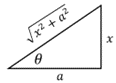
\includegraphics{images/trigsub1.png}
    \end{figure}

    From the triangle, \(\tan{\theta}=\frac{x}{a}\), meaning \(x=a\tan{\theta}\).

    Then, \(\frac{dx}{d\theta}=a\sec^2{\theta}\)

    \item 
    When \(a^2-x^2\) is embedded in the integral, label the triangle like so:
    \begin{figure}[h]
        \centering
        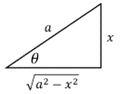
\includegraphics{images/trigsub2.png}
    \end{figure}

    From the triangle, \(\sin{\theta}=\frac{x}{a}\), meaning \(x=a\sin{\theta}\)

    Then, \(\frac{dx}{d\theta}=a\cos{\theta}\)

    \item 
    When \(x^2-a^2\) is embedded in the integral, label the triangle like so:
    \begin{figure}[h]
        \centering
        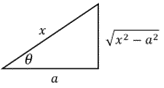
\includegraphics{images/trigsub3.png}
    \end{figure}

    From the triangle, \(\cos{\theta}=\frac{a}{x}\), meaning \(x=\sec{\theta}\)

    Then, \(\frac{dx}{d\theta}=a\sec{\theta}\tan{\theta}\)
      
    \end{enumerate}
    This quite a tricky concept so here are a couple of examples to illustrate:

    \subsection*{Example 1}
    \(\int \frac{\sqrt{25x^2-4}}{x}\,dx\)

    This is in the form \(x^2-a^2\) so we set up our triangle as so:
    \begin{figure}[h]
        \centering
        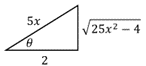
\includegraphics{images/trigsub4.png}
    \end{figure}

    \(\cos{\theta}=\frac{2}{5x}\)

    \(x=\frac{2}{5}\sec{\theta}\)

    \(dx=\frac{2}{5}\sec{\theta}\tan{\theta}\,d\theta\)

    Now we can substitute everything into our integral:

    \(\int \frac{\sqrt{25(\frac{2}{5}\sec{\theta})^2-4}}{\frac{2}{5}\sec{\theta}}\times \frac{2}{5}\sec{\theta}\tan{\theta}\,d\theta\)

    Simplifying:

    \(\int \frac{\sqrt{4\sec^2{\theta}-4}}{\frac{2}{5}}\times \frac{2}{5}\tan{\theta}\,d\theta\)

    \(\int \frac{\sqrt{4(\sec^2{\theta}-1)}}{\frac{2}{5}}\times \frac{2}{5}\tan{\theta}\,d\theta\)

    \(\int \frac{\sqrt{4\tan^2{\theta}}}{\frac{2}{5}}\times \frac{2}{5}\tan{\theta}\,d\theta\)

    \(\int 2\tan{\theta}\times \tan{\theta}\,d\theta=2\int \tan^2{\theta}\,d\theta\)

    We can’t directly integrate this, but by using the \(\tan^2{\theta}=\sec^2{\theta}-1\) identity, we can rewrite the integral and do it easily:

    \(2\int (\sec^2{\theta}-1)\,d\theta=2\tan{\theta}-2\theta+c\)

    Finally, we go back to our original triangle and write our solution in terms of x again:

    \(\tan{\theta}=\frac{\sqrt{25x^2-4}}{2}\)

    \(\theta=\cos^{-1}{(\frac{2}{5x})}\)

    \(\int \frac{\sqrt{25x^2-4}}{x}\,dx=\sqrt{25x^2-4}-2\cos^{-1}{(\frac{2}{5x})}+c\)

    \subsection*{Example 2}
    \(\int \frac{1}{x^2\sqrt{x^2+4}}\,dx\)

    This is in the form \(x^2+a^2\) so we set up our triangle like so:
    \begin{figure}[h]
        \centering
        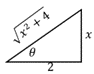
\includegraphics{images/trigsub5.png}
    \end{figure}

    \(\tan{\theta}=\frac{x}{2}\)

    \(x=2\tan{\theta}\)

    \(dx=2\sec^2{\theta}\,d\theta\)

    Substituting into the integral:

    \(\int \frac{1}{4\tan^2{\theta}\sqrt{4\tan^2{\theta}+4}}2\sec^2{\theta}\,d\theta\)

    We can simplify the root:

    \(\sqrt{4\tan^2{\theta}+4}=\sqrt{4(\tan^2{\theta}+1)}=\sqrt{4sec^2{\theta)}}=2\sec{\theta}\)

    \(\int \frac{1}{4\tan^2{\theta}\times 2\sec{\theta}}2\sec^2{\theta}\,d\theta\)

    \(\int \frac{\sec{\theta}}{4\tan^2{\theta}}\,d\theta\)

    A bit of rearranging is now required to get this into a nice integral:

    \(\frac{1}{4}\int \frac{1}{\cos{\theta}}\times \frac{\cos^2{\theta}}{\sin^2{\theta}}\,d\theta\)

    \(=\frac{1}{4}\int \frac{\cos{\theta}}{\sin^2{\theta}}\,d\theta\)

    \(=\frac{1}{4}\int \csc{\theta} \cot{\theta}\,d\theta\)

    \(=-\frac{1}{4}\csc{\theta}+c\)

    Finally, putting it back into terms of x:

    Remembering that \(\csc{\theta}=\frac{1}{\sin{\theta}}\)

    \(\int \frac{1}{x^2\sqrt{x^2+4}}\,dx=-\frac{1}{4}\csc{\theta}=-\frac{1}{4}\times \frac{\sqrt{x^2+4}}{x}=-\frac{\sqrt{x^2+4}}{4x}+c\)

    
\pagebreak

\subsection*{Questions}
(Answers - page \pageref*{Trig subs answers})
\label{Trig substitution}
\begin{enumerate}
    \item 
    \(\int \sqrt{1-x^2}\,dx\)

    \item 
    \(\int \sqrt{4-9x^2}\,dx\)

    \item 
    \(\int \sqrt{1-7x^2}\,dx\)

    \item 
    \(\int \frac{\sqrt{x^2+16}}{x^4}\,dx\)

    \item 
    \(\int \frac{2}{x^4\sqrt{x^2-25}}\,dx\)

    \item 
    \(\int x^3(3x^2-4)^{\frac{5}{2}}\,dx\)

    \item 
    \(\int x^3\sqrt{4-9x^2}\,dx\)

    \item 
    \(\int \frac{\sqrt{x^2+1}}{x}\,dx\)

    \item 
    \(\int \frac{\sqrt{1-x^2}}{x}\,dx\)

    \item 
    \(\int \frac{(x^2-1)^{\frac{3}{2}}}{x}\,dx\)

    \item 
    \(\int \cos{x}\sqrt{9+25\sin^2{x}}\,dx\)

    \item 2022 Scholarship exam
    
    Show that \(\int \frac{1}{\sqrt{1+x^2}}\,dx=\ln{|\sqrt{1+x^2}+x|}+c\)
    
\end{enumerate}


\pagebreak


\end{document}